\documentclass{article}
\usepackage{graphicx}
\usepackage{color}
\title{Prelim Outline}
\author{Shivesh Pathak}

\begin{document}
\maketitle

Text in \color{blue} blue \color{black} are things that need to be planned.

\section{Motivation/Background}
\begin{enumerate}
\item We want to construct an accurate low-energy model Hamiltonian for the cuprates.
\item Hole doped cuprates have been studied for a long time, and the relevant degrees of freedom are both O p and Cu d orbitals. 
\item Electron doped cuprates are less studied and we believe they are simpler since the O p orbitals should play a much smaller role.
\item We plan on building an low-energy model for the electron doped cuprate SrCuO$_2$ using a density-matrix downfolding method and accurate many-body QMC calculations.
\end{enumerate}

\section{Preliminary calculations: DFT}
\subsection{Undoped (x=0)}
\begin{enumerate}
\item We did eight unit cell DFT calculations with a PBE0 functional to calculate the energies of states with singly occupied Cu d$_{x^2-y^2}$ orbitals but with different spin textures.

\item We mapped these states onto spin-1/2 local moment states and used to fit to an AFM Heisenberg model:
$$H_m = J\sum_{ij} \frac{1}{2} \vec{S_i}\cdot\vec{S_j} $$ 

\item The results of this fitting on seven different spin textures yields good results for two different basis sets (BFD Cutoff, BFD PBC 0.2).

\item For every SCF calculation done the BFD PBC 0.2 basis set had higher total energy than the BFD Cutoff, so I will only present results for the Cutoff basis set.

\item The high $R^2$ values of the fit indicates that a simple AFM Heisenberg model should be sufficient to capture the low-energy behavior of undoped SrCuO$_2$.
\end{enumerate}

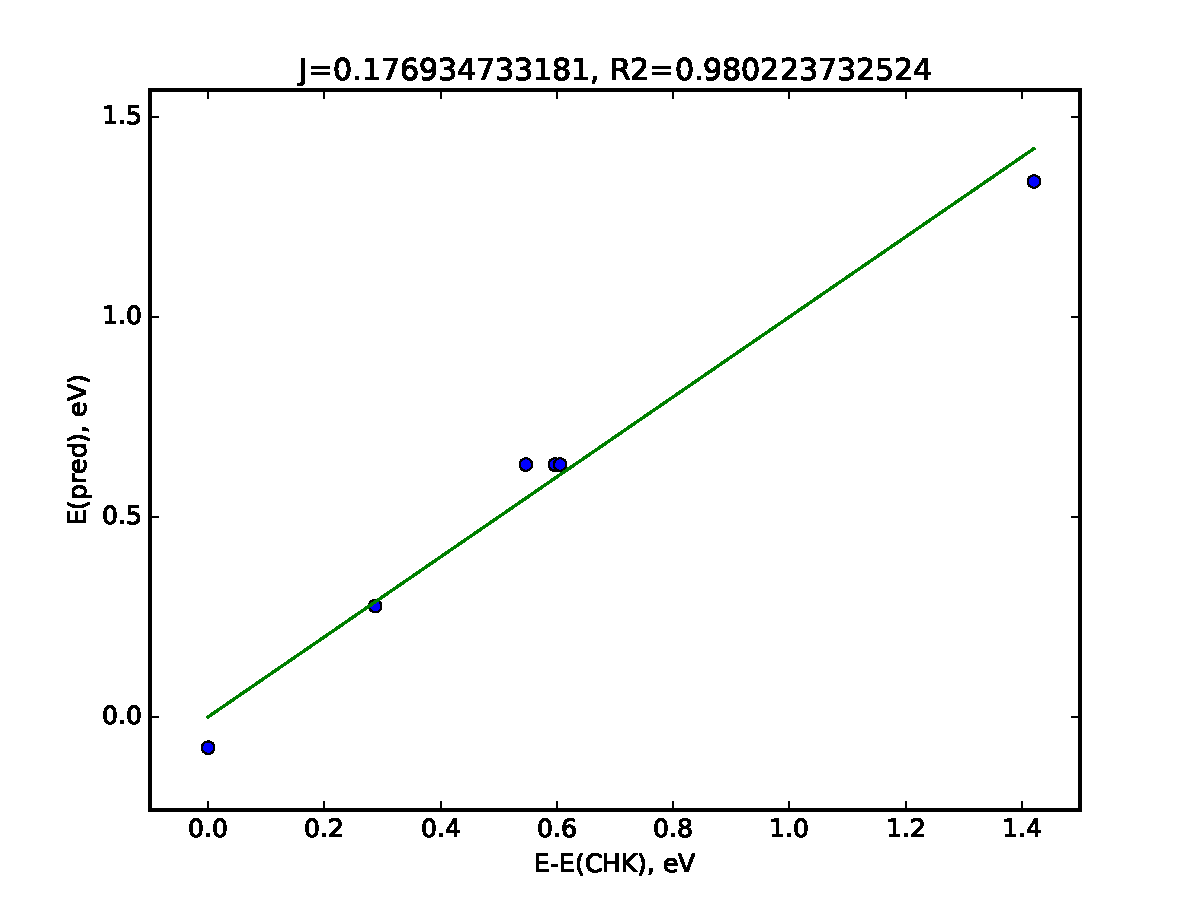
\includegraphics[width=0.5\textwidth]{../undoped/PBE0_8/J_fit_naive.pdf}

\subsection{Overdoped (x=0.25)}
\begin{enumerate}
\item We similarly did seventeen x=0.25 doped calculations in PBE0, from which we got four low energy states. 

\item Similarly to the x=0 calculations, the x=0.25 PBE0 calculations yielded lower total energy for the BFD Cutoff basis. All results shown are for that basis.

\item Low-energy is defined as states with energy less than 0.3 eV from the lowest energy state we had, a collinear doped state.

\item We used the band structures and total energies of these four low energy states to fit to a naive model with $t, t^\prime, K, J$ parameters: NN-hopping, NNN-hopping, NN-Kondo term, and NN-Heisenberg-AFM term

$$H_m =  -t\sum_{\langle i, j \rangle, \sigma} (c_{i\sigma} ^\dagger c_{j\sigma} + h.c.) + 
t^\prime\sum_{\langle\langle i, j \rangle\rangle, \sigma} (c_{i\sigma} ^\dagger c_{j\sigma} + h.c.) + $$ 
$$K \sum_{\langle i, j \rangle} \vec{S_i} \cdot c_{j\alpha}^\dagger \vec{\sigma}_{\alpha \beta} c_{j\beta} + J\sum_{ij} \frac{1}{2} \vec{S_i}\cdot\vec{S_j} $$ 

\item We map each of the PBE0 states into the model Hilbert space by breaking the occupied bands into a) fully occupied and b) partially occupied. 

\item The orbitals from a) then build a spin density that defines the variables $\vec{S_i}$ and the orbitals from b) define the variables $c_i^\dagger$.

\item We then create a single body  Hamiltonian where we treat the spins $\vec{S_i}$ as a fixed background upon which the itinerant $c_i^\dagger$ electrons can move. 

\item We solve this model Hamiltonian and fit to the PBE0 band structure and further compare the total energy of the model to the PBE0 total energy.

\item Since we are fitting to two different quantities we used a Pareto efficiency analysis to get the best balance between a fit to total energy and a fit to band structure. 

\item The cost function is shown below, and $w_E$ varies in the plot shown below.

$$Cost = w_E|E_m - E_{PBE0}|^2 + \sum_{|k|\le k_F} |e_{m,k} - e_{PBE0,k}|^2$$

\item In the fitting we hold the value of $J=0.178$ eV fixed as a prior, which is the optimal value from the x=0 fit. \textcolor{red}{Why?}
 
\item We find that the most efficient point is at the blue square on the Pareto plot. Below we plot the fit to the band structure and comparison of the model and PBE0 total energies. 

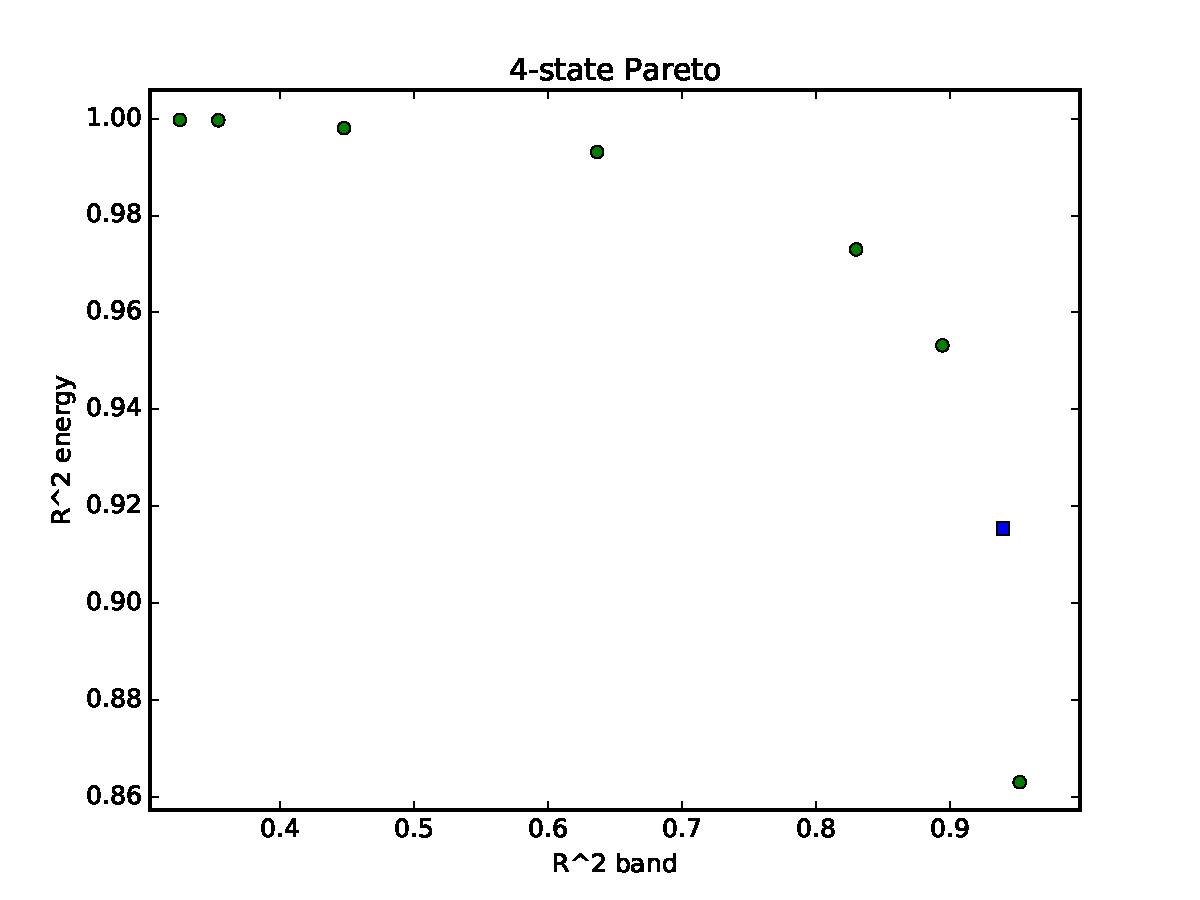
\includegraphics[width=0.5\textwidth]{../doped_fv/PBE0_8/tb_fit_0p25/pareto4.pdf}
\linebreak

\color{black}

\item The parameter values at this point on the Pareto plot are $t,t^\prime,K,J=  1.04, 0.53, -0.15, 0.178 $eV.

\item Below is a figure with a fit to the total energies and band structure.

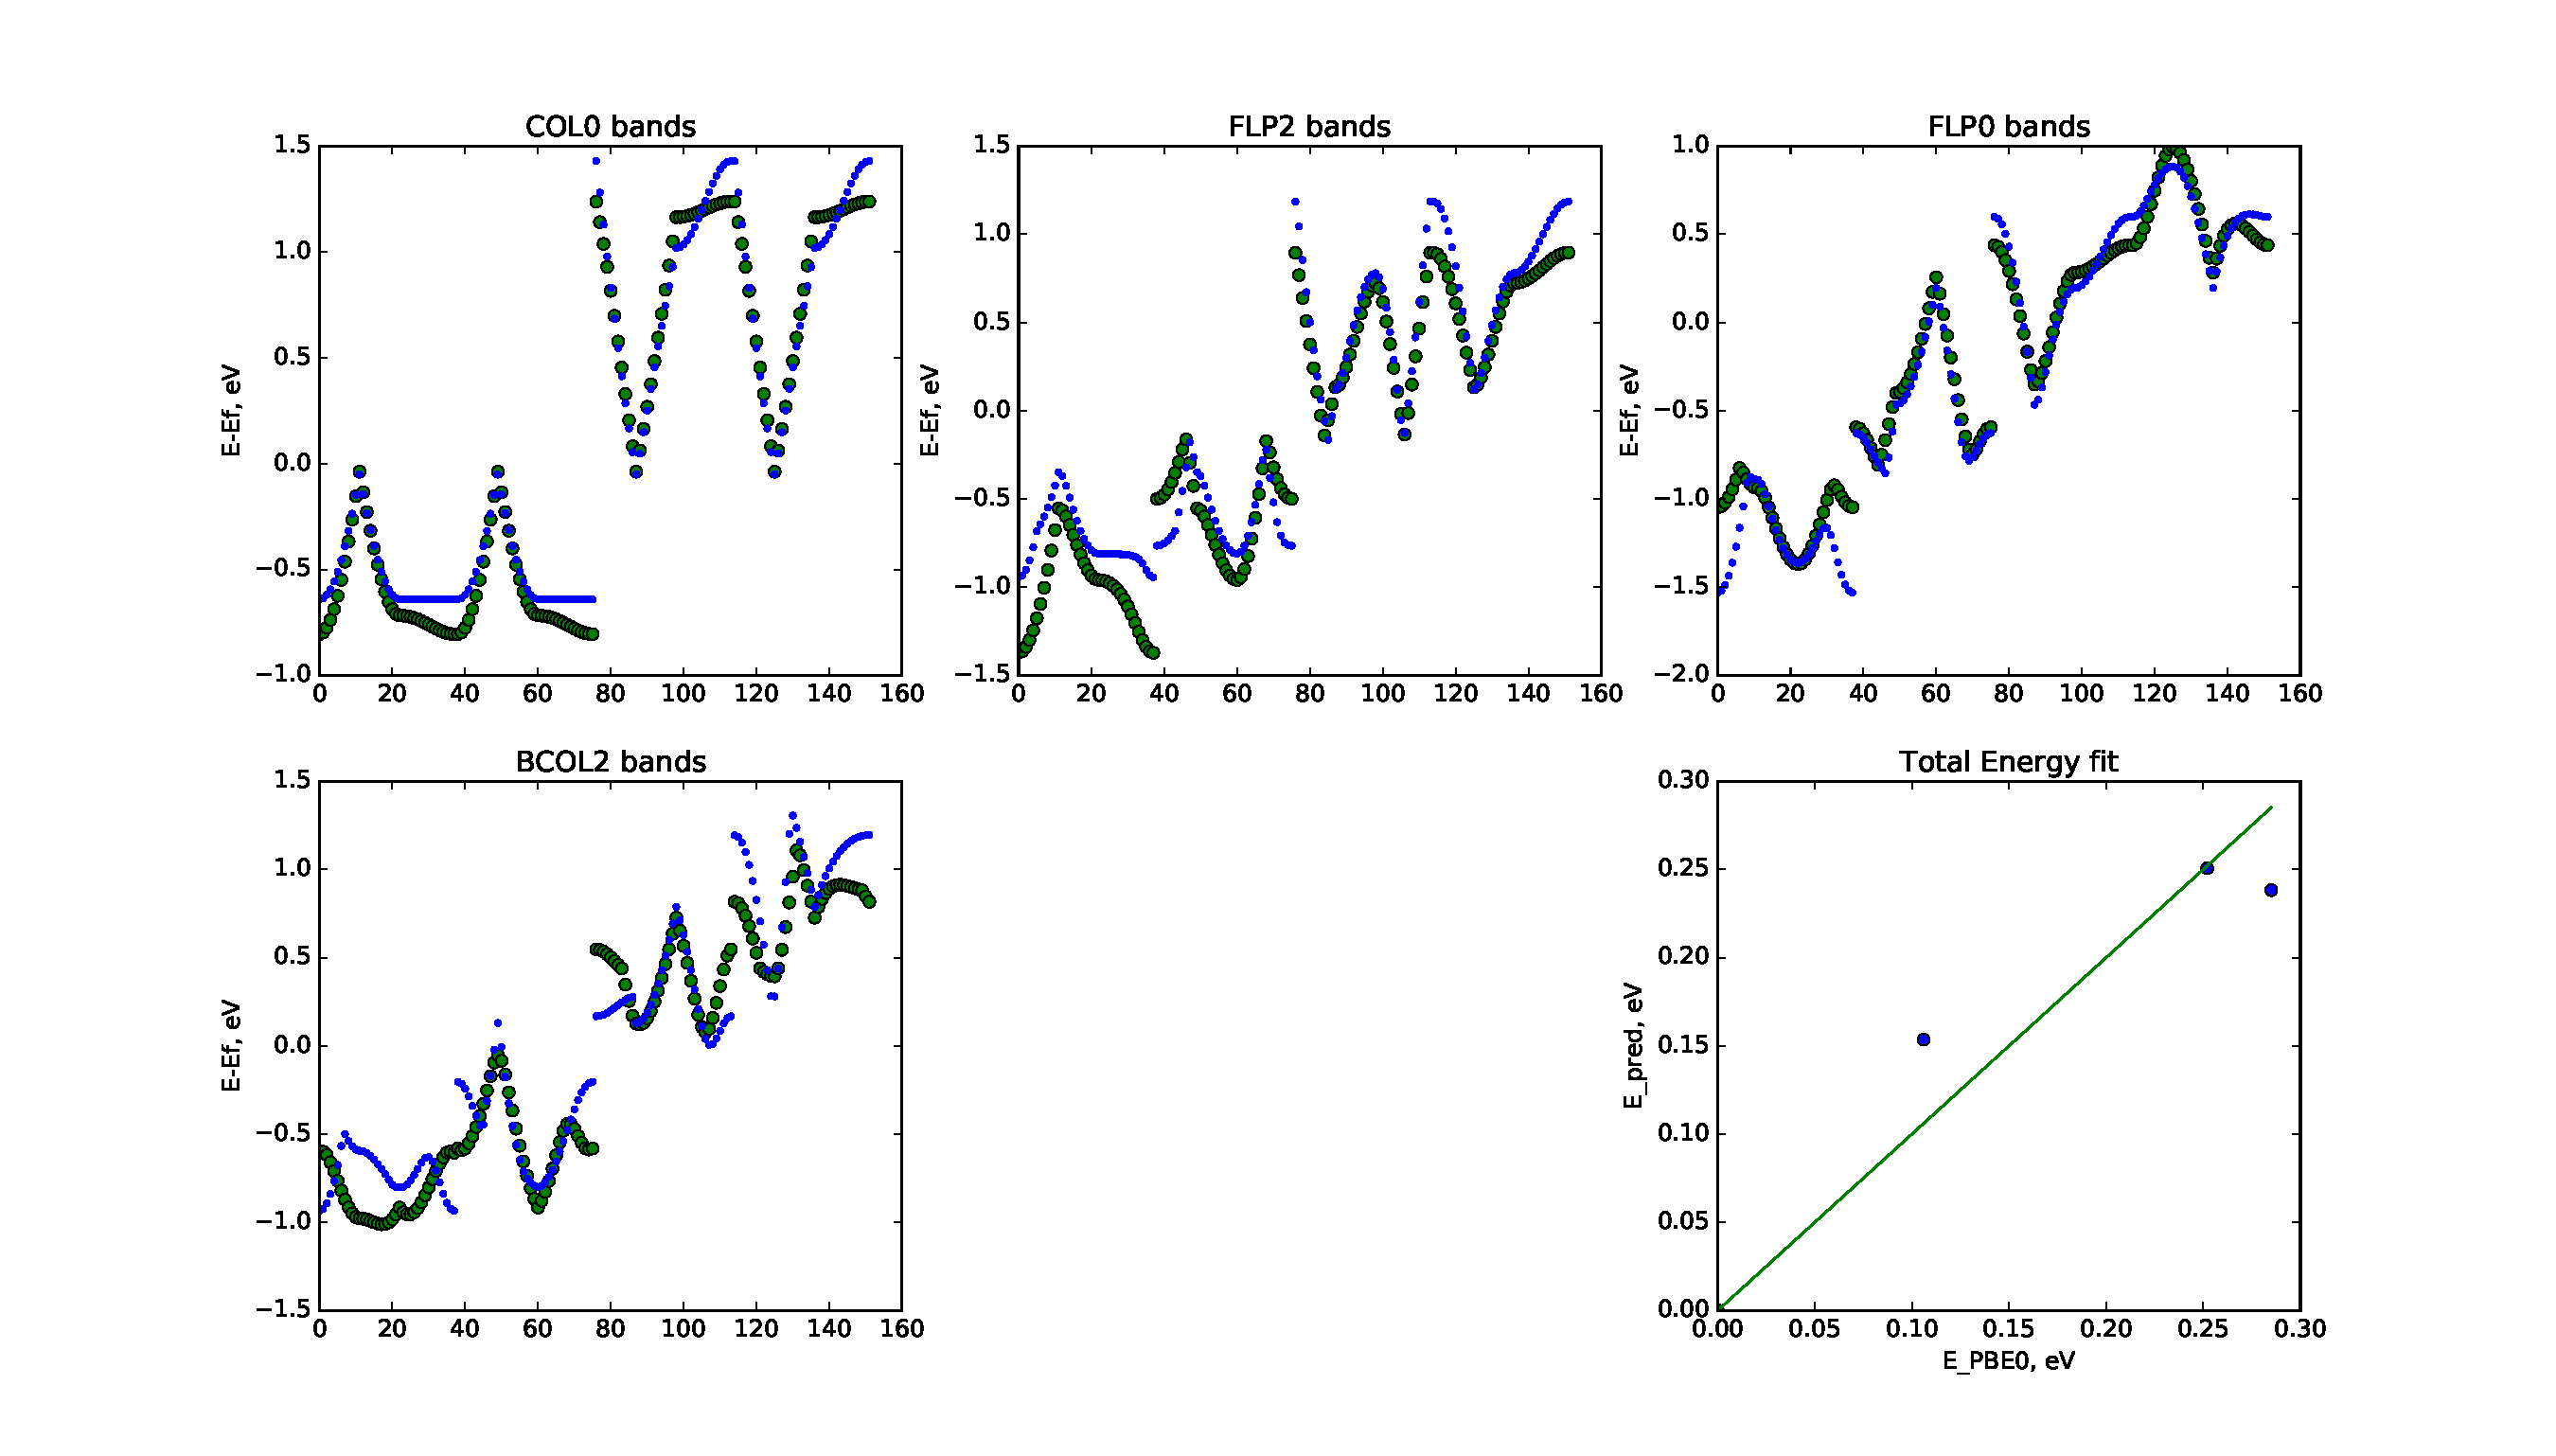
\includegraphics[width=0.7\textwidth]{../doped_fv/PBE0_8/tb_fit_0p25/pareto4_low.pdf}
\end{enumerate}

\subsection{(Near) optimally doped (x=0.125)}
\begin{enumerate}
\item The fitting for x=0.125 is identical to x=0.25 except that the states in PBE0 we use are different.

\item As we had for the x=0.25 calculation, we got four low energy states for x=0.125, and all results below are for the BFD Cutoff basis.

\item Below is the Pareto efficiency plot using the four low energy x=0.125 states and using the cost function from before. The blue square is the point we chose as most efficient.

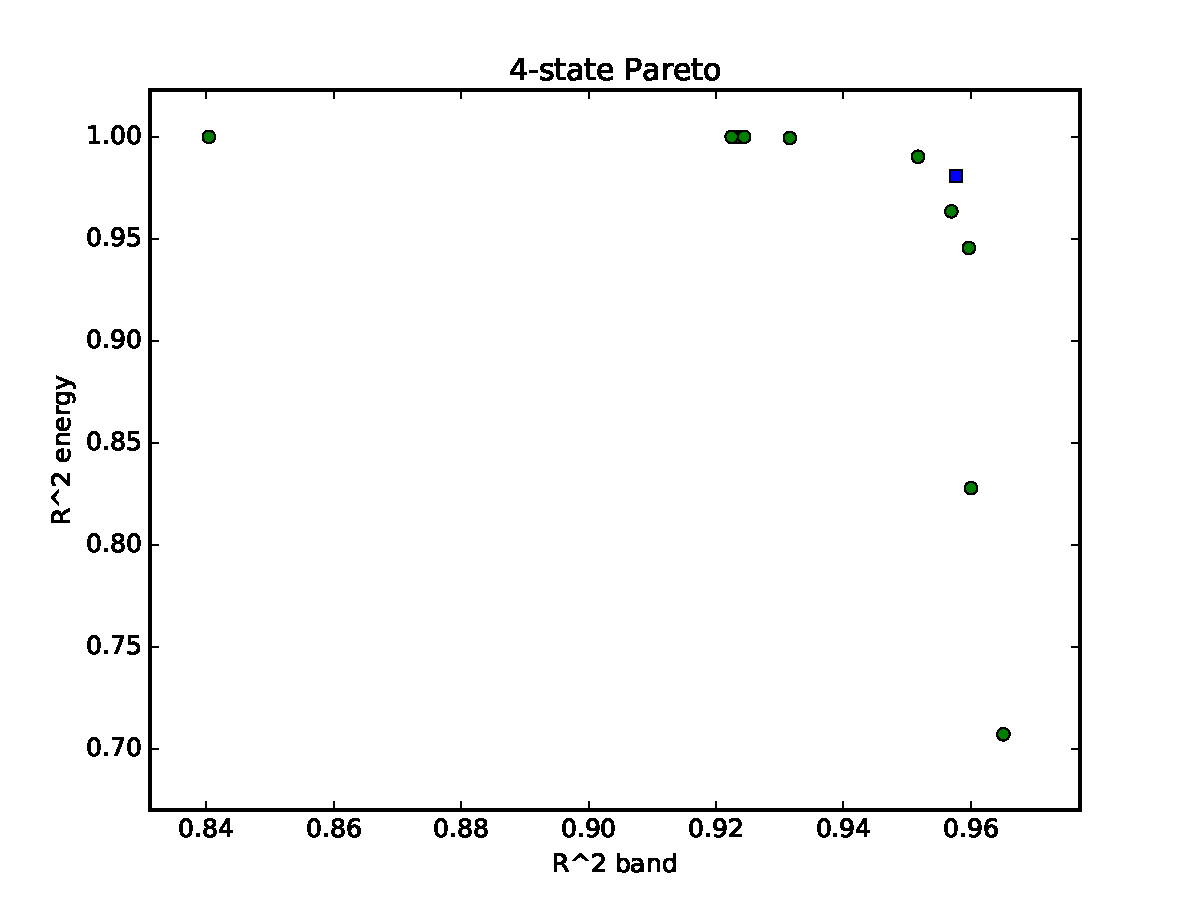
\includegraphics[width=0.5\textwidth]{../doped_fv/PBE0_8/tb_fit_0p125/pareto4.pdf}
\linebreak

\item The parameter values at this point on the Pareto plot are $t,t^\prime,K,J=  1.15,  0.39, -0.29, 0.18 $eV.

\item Below is a figure with a fit to the total energies and band structure.

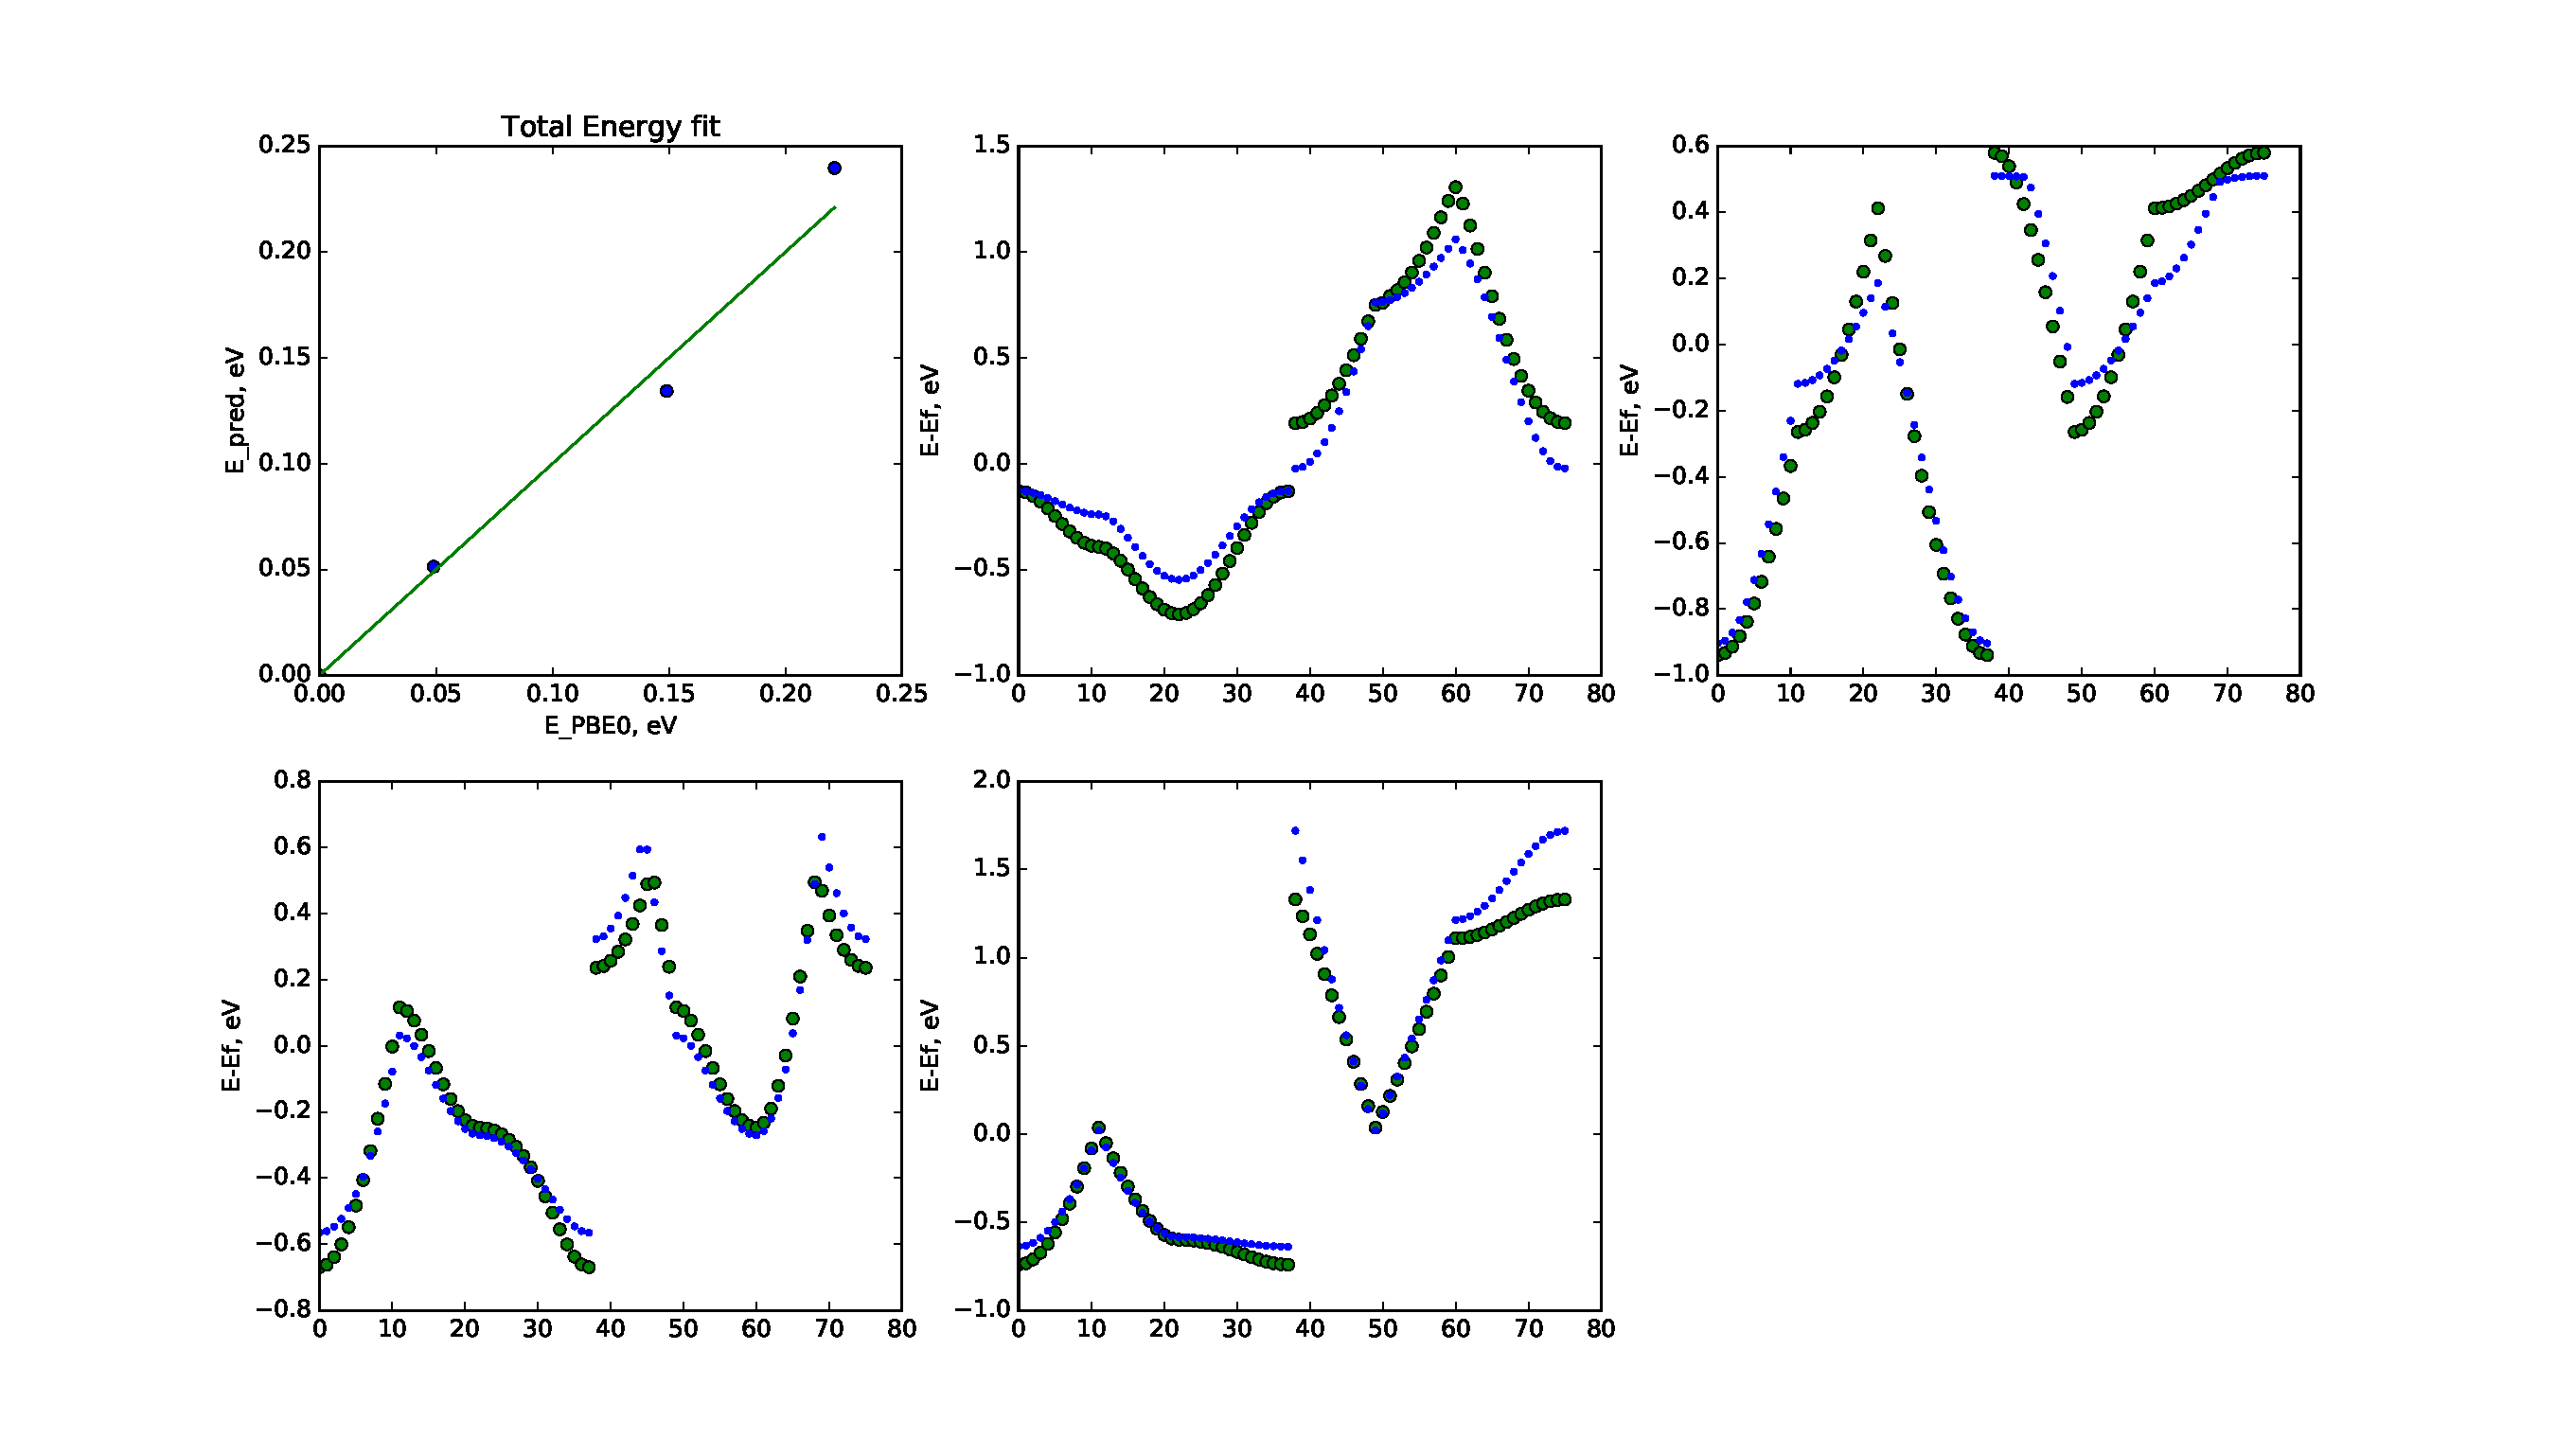
\includegraphics[width=0.7\textwidth]{../doped_fv/PBE0_8/tb_fit_0p125/pareto4_sel.pdf}
\end{enumerate}

\subsection{Conclusions}
\begin{enumerate}
\item Fitting to our PBE0 results provides some evidence that our low energy model with four terms $t, t^\prime, K, J$ may describe the low energy Hilbert space of SrCuO$_2$ accurately.

\item The table below shows the variation in the model parameters under doping, in eV.

\begin{center}
\begin{tabular}{ c c c c c }
Doping & t & t$^\prime$ & K & J \\ 
\hline
x=0 & 0 & 0 & 0 & 0.178 \\
x=0.125& 1.15&  0.39& -0.29& 0.178 \\
x=0.25 & 1.04& 0.53& -0.15&0.178 \\
\end{tabular}
\end{center}

\item This fitting was preliminary and is not a systematic or rigorous fitting procedure. 

\item My thesis project will be based to use the density matrix downfolding procedure to conduct a more rigorous version of model fitting.
\end{enumerate}

\section{Density matrix downfolding (DMD) calculations}
\subsection{Basis}

\begin{enumerate}
\item In order to do our DMD calculations we need a single particle basis to evaluate the density matrix on.  We use intrinsic atomic orbitals (IAOs) as our one particle basis.

\item \textbf{Undoped (x=0)}]
\begin{enumerate}
\item Shown below are the occupations of different IAOs for the checkerboard spin textured PBE0 state. 

\item The IAOs show that the primary variation between occupation is in the spin of an unpaired electron in the $3d_{x^2-y^2}$ orbital. 

\item The oxygen orbitals do not play a significant role.

\item Another important feature is that for each copper atom there are TWO $3d_{x^2-y^2}$ IAOs: one for the majority spin and one of the minority spin.

\end{enumerate}
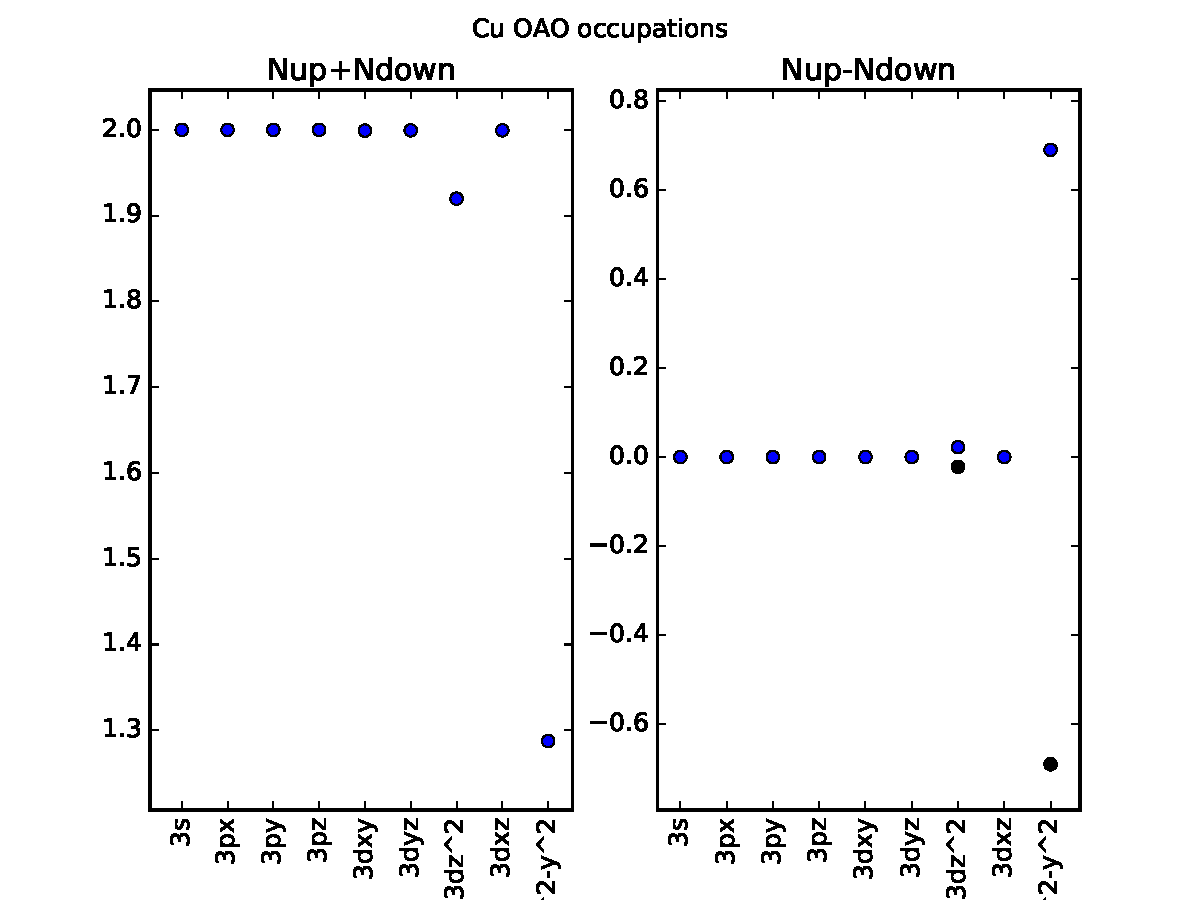
\includegraphics[width=0.5\textwidth]{../undoped/PBE0_8/CHK/dens_iao2_cu.pdf}
\linebreak

\item \textbf{Overdoped (x=0.25)}
\begin{enumerate}
\item For the doped calculation, we did the same IAO analysis as for the x=0 case. 

\item Unlike the x=0 case, once doped the occupation number changes as well as the spin. 

\item Below is shown the difference in occupation of the spin-down and spin-up $3d_{x^2-y^2}$ orbitals of the doped collinear state MINUS to the undoped collinear state. 

\item The occupation of the dominant primary channel does not vary but that of the the secondary spin channel does.

\item We can therefore attribute the prior orbitals to to the fixed magnetic moments and the latter to the itinerant electrons.

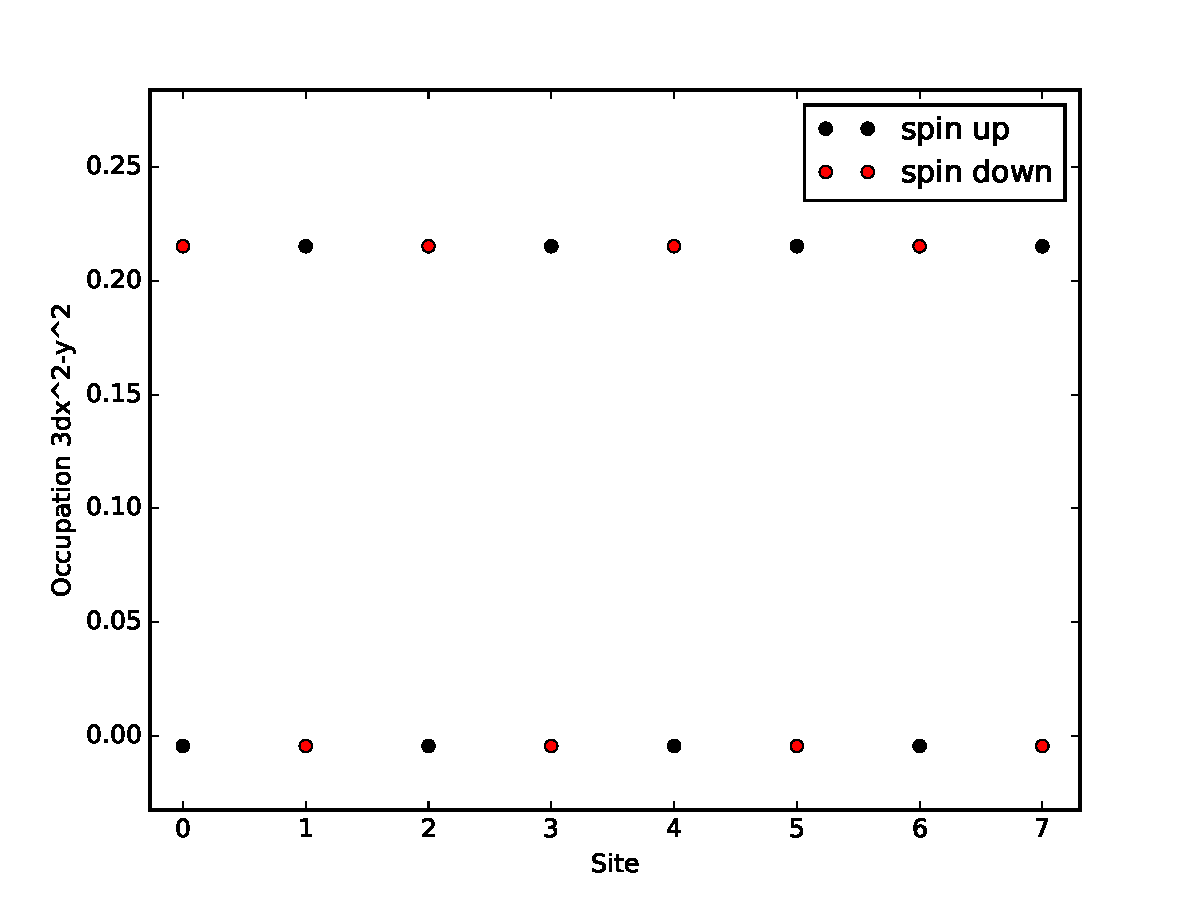
\includegraphics[width=0.5\textwidth]{../doped_fv/PBE0_8/COL0/iao/sub_occd.pdf}

\item We find that the majority spin IAOs relax in a localized manner with on site $d_{x^2-y^2}$ character, while the minority spin IAOs relax with $O p$ character across the calculation cell.

\includegraphics[width=0.5\textwidth]{../doped_fv/PBE0_8/COL0/iao/DIFF_0_10.pdf} 
\linebreak

\includegraphics[width=0.5\textwidth]{../doped_fv/PBE0_8/COL0/iao/DIFF_0_810.pdf}

\item The orbital corresponding to the primary spin channel will be used to calculate DM elements of the fixed spin moments $\vec{S_i}$ and the secondary spin channel IAO will be used to calculate DM elements of the itinerant electrons $c_i^\dagger$
\end{enumerate}

\item \textbf{Optimally doped (x=0.125)}
\begin{enumerate}
\item The IAO analysis yields the same conclusions as the overdoped case.

\item Shown below is the difference in occupation of the spin-down and spin-up 3$d_{x^2-y^2}$ orbitals of the doped flip state MINUS the undoped flip state.

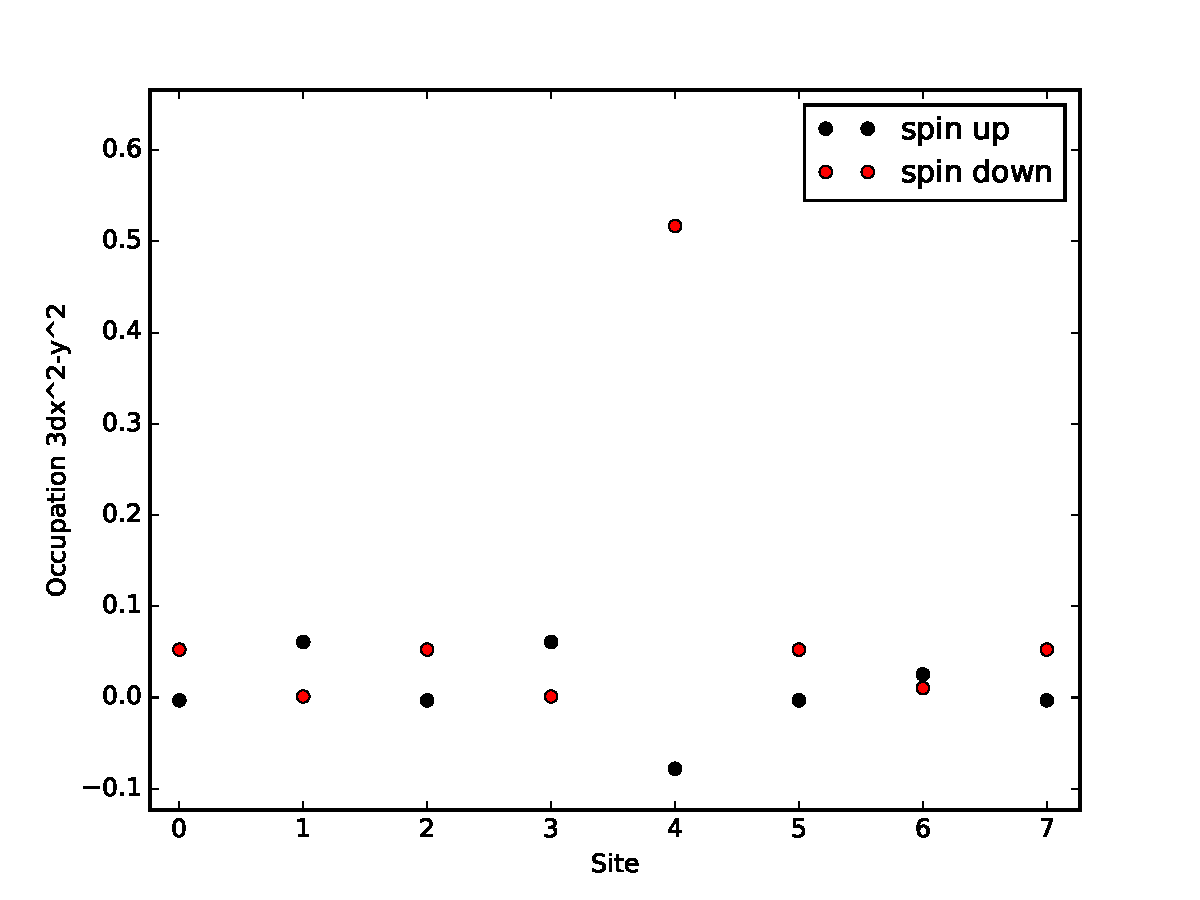
\includegraphics[width=0.5\textwidth]{../doped_fv/PBE0_8/FLP1/iao/sub_occd.pdf}
\linebreak

\includegraphics[width=0.5\textwidth]{../doped_fv/PBE0_8/FLP1/iao/DIFF_0_50.pdf} 
\linebreak

\includegraphics[width=0.5\textwidth]{../doped_fv/PBE0_8/FLP1/iao/DIFF_0_850.pdf}

\end{enumerate}
\end{enumerate}

\color{blue}
\subsection{Low energy states}
\begin{enumerate}
\item \textbf{Undoped (x=0)} For the undoped calculations, we have seven different spin textures. We can just use these for the model fitting since we will be fitting to a single parameter, $J$.

\item \textbf{Overdoped (x=0.25)}
\begin{enumerate}
\item We have four low energy states for x=0.25. We will use these four states, as well as states that are singles (maybe double) excitations above these four states. Only states with energy lower than our cutoff will be used.
\item We can also take linear combinations of states with singles and double excitations. This can help us generate many more states and also increase our fitting efficiency since we can then make use of parameter derivatives w.r.t the determinant coefficients.
\end{enumerate}

\item \textbf{(Near) optimally doped (x=0.125)}
\begin{enumerate}
\item Same as x=0.25.
\end{enumerate}
\end{enumerate}

\subsection{K-points}
\begin{enumerate}
\item \textbf{Undoped (x=0)} For the undoped calculations, a $\Gamma$ point calculation should be sufficient to resolve any finite size effects because we have a large unit cell for calculation and the system is strongly insulating.

\item \textbf{Doped (x=0.25, 0.125)}
\begin{enumerate}
\item For the doped calculations our first goal will be to do calculations just on the $\Gamma$ point, since this should give us a good sense of whether the model we are interested in makes sense or not.

\item We can consider doing other k-point (twist boundary) calculations if we think that the finite size errors on the calculations at a single twist are too large.
\end{enumerate}
\end{enumerate}

\subsection{QMC workflow}
for x=0, 0.125, 0.25 \\
\indent for k-points from section (3) \\ 
\indent \indent for states from section (2) \\
\indent \indent \indent Take lowest energy Slater det, variance optimize Jastrow;\\
\indent \indent \indent use this Jastrow for all following calculations
\\

\indent \indent \indent Calculate 1/2-RDM and quantities for parameter derivative fitting \\ 
\indent \indent \indent using FN-DMC for basis elements in section (1)\\

\noindent Conduct fitting to $t,t^\prime, K,J$ model using DMD method with parameter derivative fitting. \\

\noindent Alter k-points, states from sections (3) and (2) as necessary for calculation.  



\end{document}